\documentclass[10pt,a4paper]{article}

\usepackage{enumerate}
\usepackage[top=2in, bottom=1.5in, left=1in, right=1in]{geometry}
\usepackage{fancyhdr} 		% page header
\usepackage{listings} 		% present source code.
\usepackage{amsmath}
\usepackage{amssymb}
\usepackage{float}
\usepackage{graphicx}
\usepackage{epstopdf}
\usepackage{hyperref}
\usepackage{lipsum}			% just to generate text for the example

\pagestyle{fancy} 
\fancyhf{}
\fancyhead[L]{CS 540-1}
\fancyhead[R]{Fall 2018}

\def\x{\mathbf{x}}
\def\y{\mathbf{y}}
\def\w{\mathbf{w}}
\def\p{\mathbf{p}}

\begin{document}
\begin{center}
{\bf \large CS 540-1: Introduction to Artificial Intelligence

Homework Assignment \# 3

\vspace{0.5cm}

Assigned:  9/20 

Due:  9/27 before class} 
\end{center}

\section*{Question 1: The Flying Klotski [100 points]}
This is a programming question. The solution to the programming problem should be coded in Java, {\bf and you are required to use only built-in libraries} to complete this homework. Please submit a single zip file named hw3.zip, which should contain a source code file named {\bf Klotski.java} with no package statements, and make sure your program is runnable from command line on a department Linux machine. 
We provide a skeleton Klotski.java code that you can optionally use, or you can write your own.

The goal of this assignment is to become familiar with A* search. The assignment tests your understanding of AI concepts, and your ability to turn conceptual understanding into a computer program. All concepts needed for this homework have been discussed in class, but there may not be existing pseudo-code for you to directly follow.

\href{https://en.wikipedia.org/wiki/Klotski}{Klotski} is a sliding block puzzle thought to have originated in the early 20th century. 
Ten pieces (colored) are placed inside a $5\times4$ box,
among them one $2\times2$ block, four $2\times1$ blocks, one $1\times2$ block and four $1\times1$ blocks. 
The empty spaces are white.
The following is a possible initial state $S_1$:

\centerline{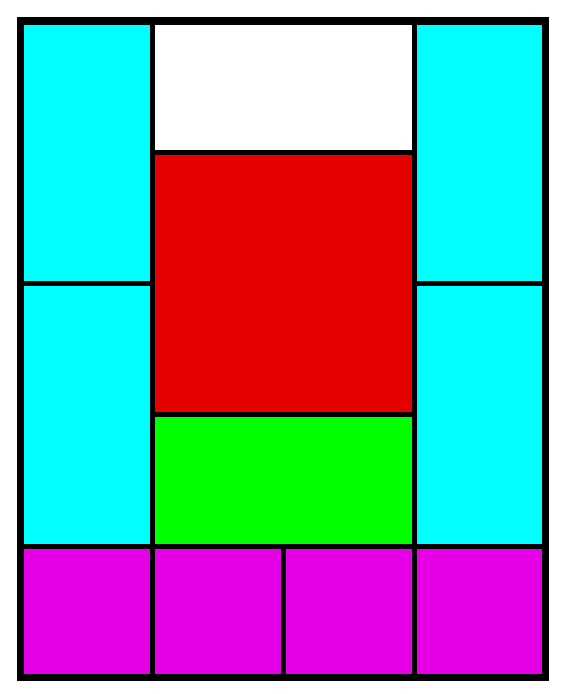
\includegraphics[width=0.18\textwidth]{figure_1.eps}}

Our rules for Klotski is slightly different from the original ones. 
The player is not allowed to remove blocks. 
Except for $1\times1$ blocks, larger blocks can only move horizontally or vertically one square at a time. 
So $S_1$ has this successor by moving the $2\times 2$ block:

\centerline{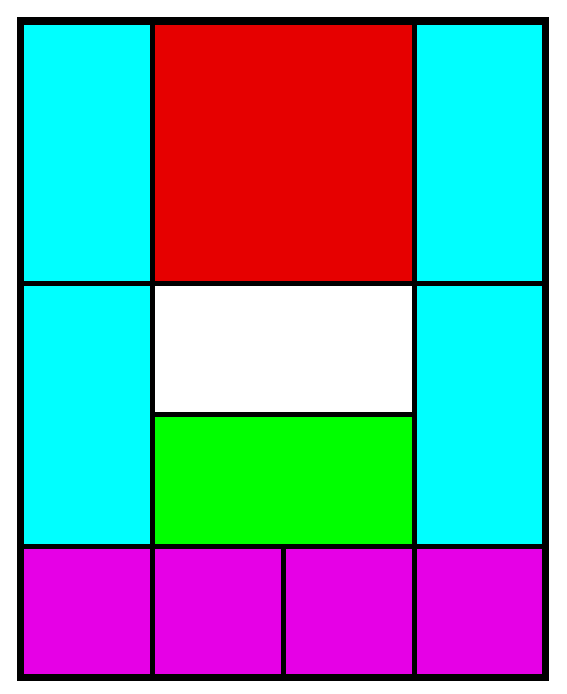
\includegraphics[width=0.18\textwidth]{figure_2.eps}}

However, we allow a $1\times1$ block to \emph{fly} to any empty space, no matter if the empty space is adjacent to it or not. 
This also counts as one move.
Because of this new rule, $S_1$ has 8 additional successors by flying a $1\times1$ block:

\centerline{
    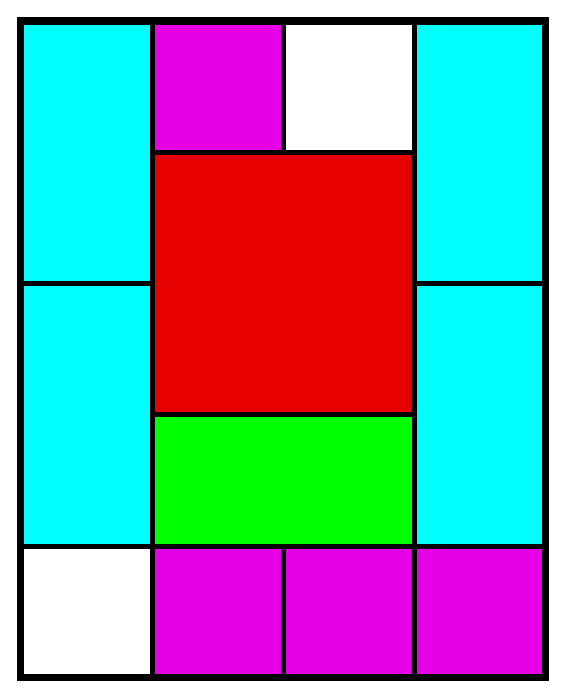
\includegraphics[width=0.18\textwidth]{figure_3.eps}
    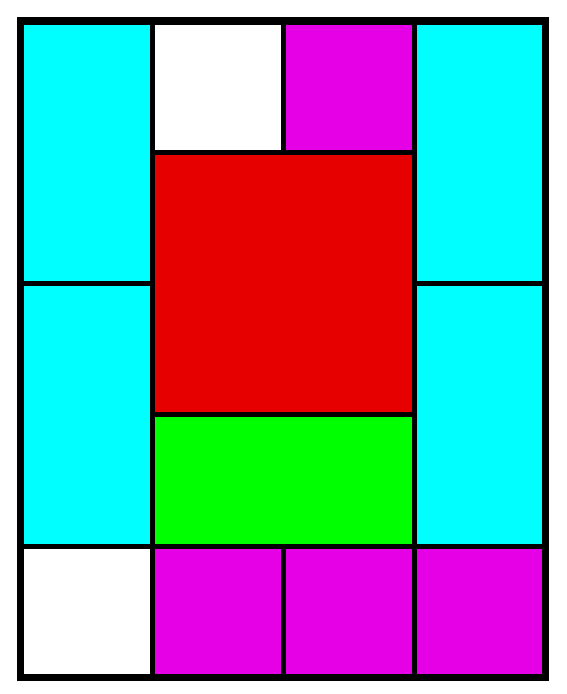
\includegraphics[width=0.18\textwidth]{figure_4.eps}
    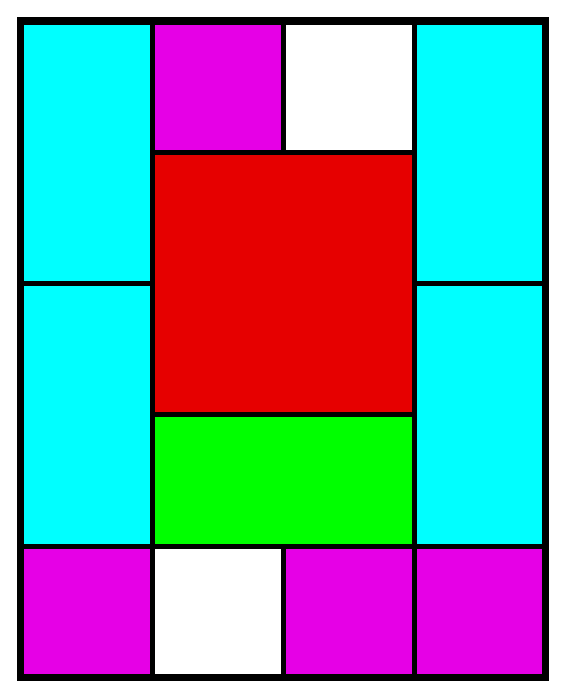
\includegraphics[width=0.18\textwidth]{figure_5.eps}
    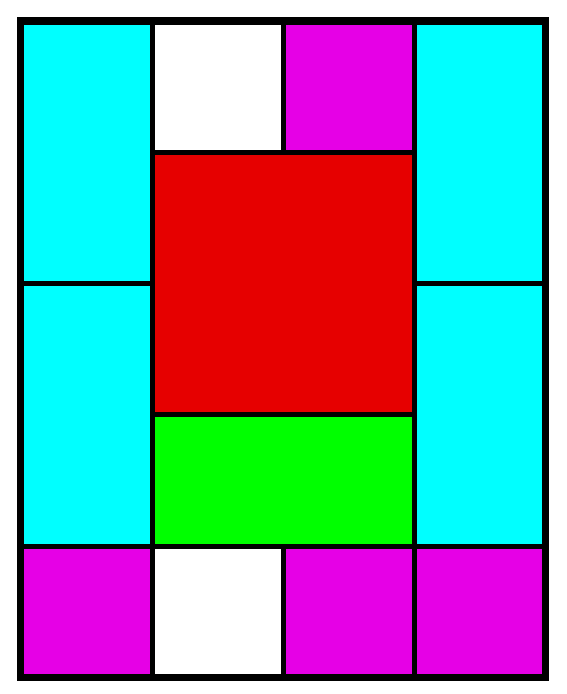
\includegraphics[width=0.18\textwidth]{figure_6.eps}
}
\centerline{
    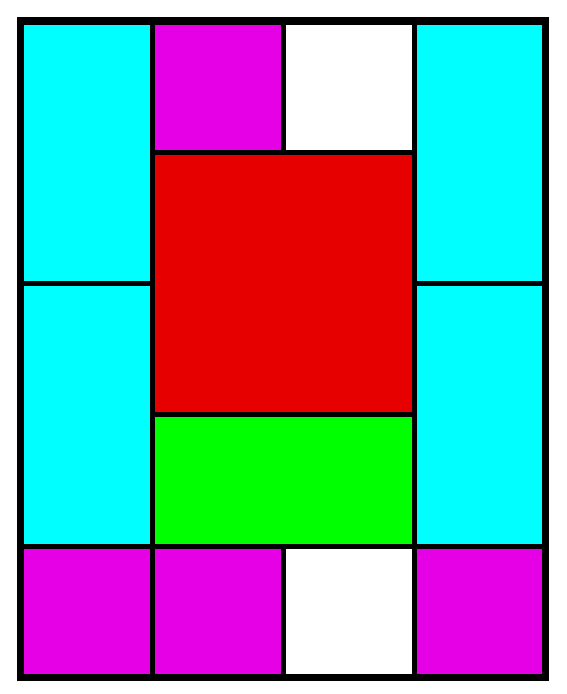
\includegraphics[width=0.18\textwidth]{figure_7.eps}
    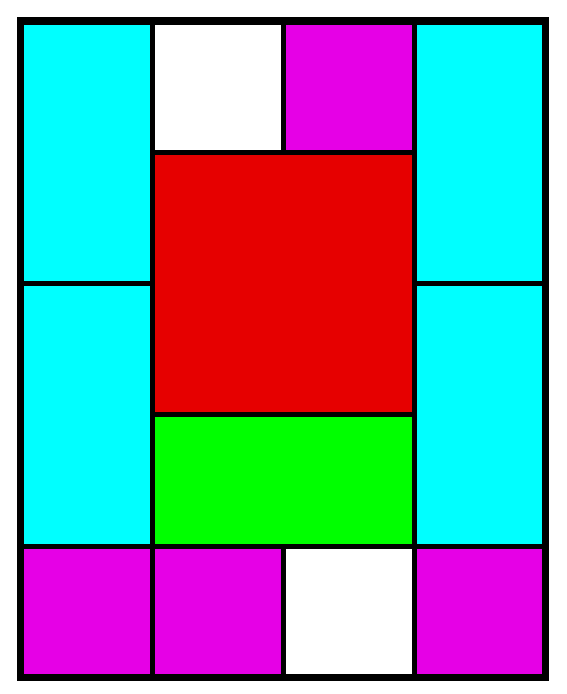
\includegraphics[width=0.18\textwidth]{figure_8.eps}
    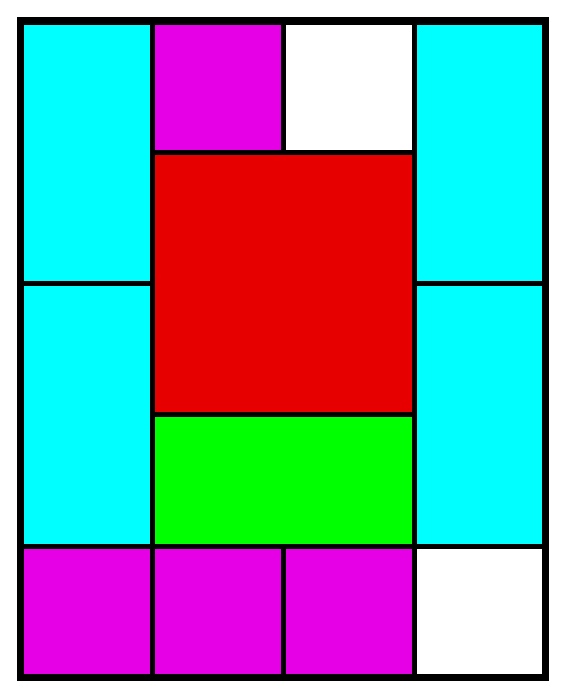
\includegraphics[width=0.18\textwidth]{figure_9.eps}
    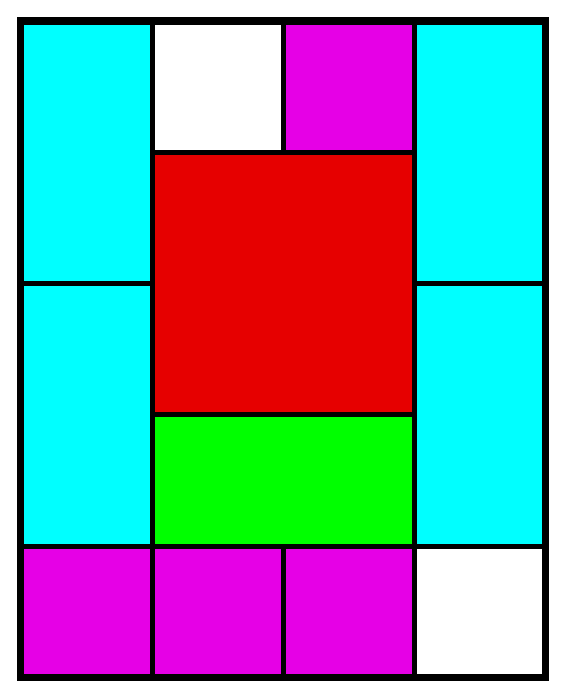
\includegraphics[width=0.18\textwidth]{figure_10.eps}
}

So $S_1$ has 9 successors in all. 

Let us look at another example with a different state $S_2$:

\centerline{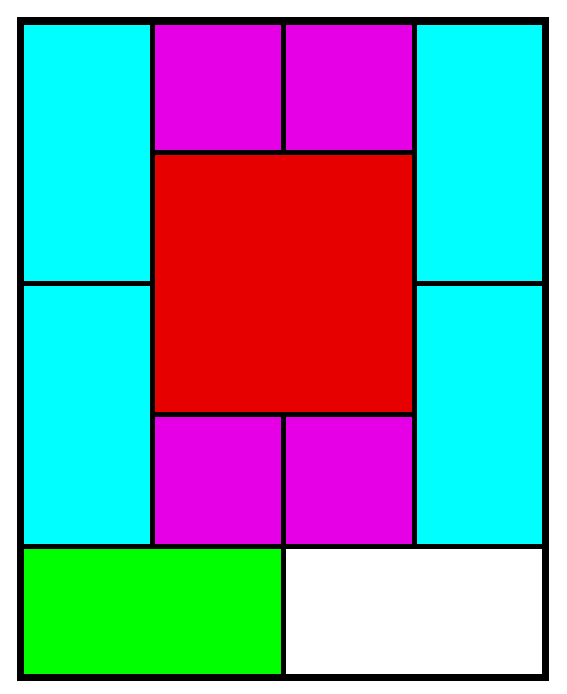
\includegraphics[width=0.18\textwidth]{figure_11.eps}}

To emphasize, larger blocks can only move by one square in one step.
This is a valid successor of $S_2$: 

\centerline{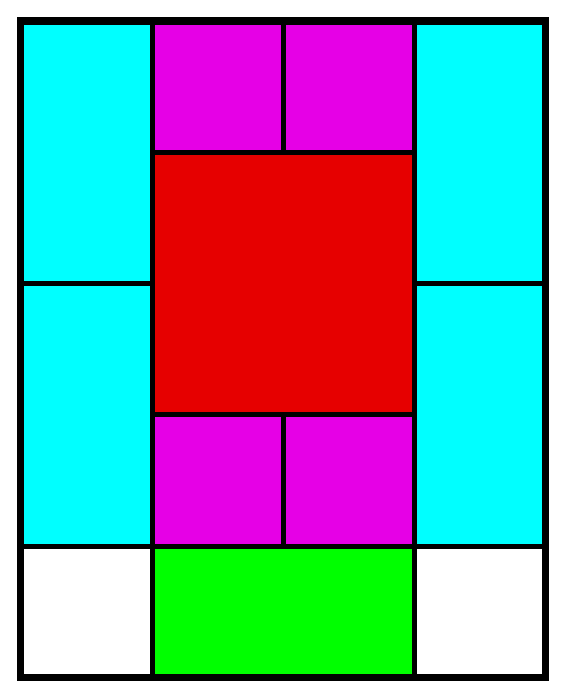
\includegraphics[width=0.18\textwidth]{figure_12.eps}}

But this is not:

\centerline{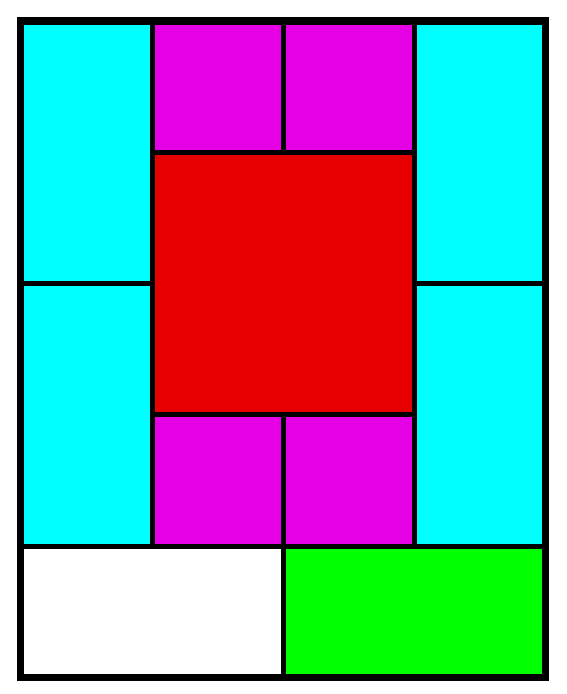
\includegraphics[width=0.18\textwidth]{figure_13.eps}}

Of course, $S_2$ has 8 additional successors resulting from flying the $1\times 1$ blocks, and one more successor by sliding down the lower right cyan block.

The goal of the game is to move the $2\times2$ red block to the center of the lowest row (the ``exit''):
We do not care about the position of other blocks (omitted in the gray area).
Therefore, you have a simple goal test that corresponds to multiple goal states:

\centerline{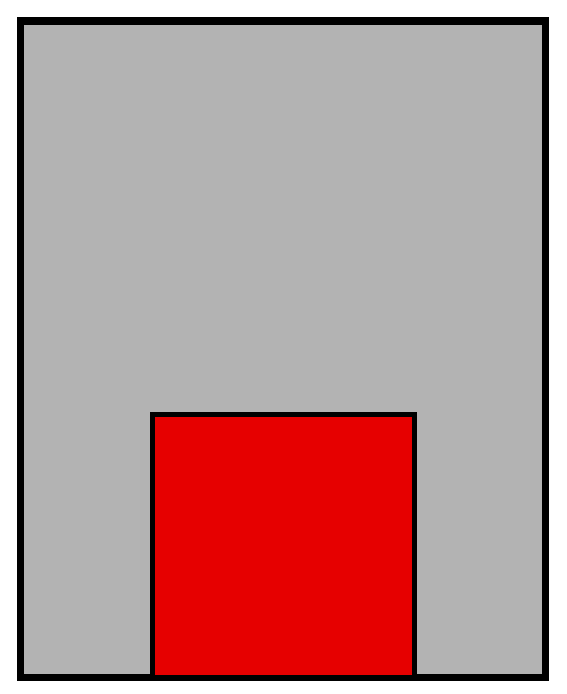
\includegraphics[width=0.18\textwidth]{figure_14.eps}}



For this question, you will use A* search to find the shortest path from an initial state to a goal state. 
Write a program {\bf Klotski.java} with the following command line format:

\begin{verbatim}
    $java Klotski FLAG tile1 tile2 tile3 ... tile20
\end{verbatim}

FLAG is an integer that specifies the behavior and output of the program (see below). 
In the command line, tile1 -- tile20 specify the initial state in the natural reading order (left to right, top to bottom). 
We use 0 to represent empty block, 1 to represent $2\times2$ block, 2 to represent $2\times1$ block, 3 to represent $1\times2$ block and 4 to represent $1\times1$ block.
For example, 
the following command line 

\begin{verbatim}
    $java Klotski 100 2 4 4 2 2 1 1 2 2 1 1 2 2 4 4 2 0 0 3 3
\end{verbatim}

represents this initial state:

\centerline{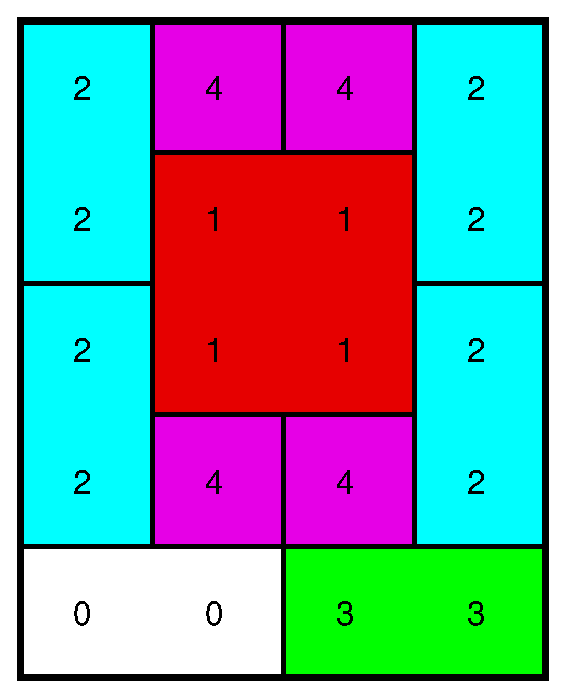
\includegraphics[width=0.18\textwidth]{figure_15.eps}}

\begin{enumerate}

\item When FLAG=100, generate, sort, and print all successors of the initial state. For each state, print 5 lines of 4 digits per line, with no space between each digit; then print an empty line. 

The successors should be sorted according to the following rule.
If we view the whole board as a 20-digit number in the natural reading order (from left to right, top to bottom), then 
print the successors sorted from small to large.
Hint: you may also implement these 20-digit integers as strings and compare them according to dictionary order.

Please see examples \verb|example*100| in the attached files; the corresponding inputs are in file \verb|input|. 

\item 
Implement A* search as defined on slide 21 of informed search (see course webpage). Use a constant heuristic function $h=0$ for all states. This reduces A* to uniform cost search. 
For tie breaking when popping from the priority queue, pop the state with the smallest 20-digit ID among states with the minimum $f$ score.

When FLAG=200, in each iteration (please see examples \verb|example*200| in the attached files; so on and so forth for other FLAGs): 
\begin{itemize}
\item right after step 3 print a line \emph{iteration i} where $i$ is the iteration number (starting from 1), then print the node $n$;
\item right after step 5 print the word \emph{OPEN}, print the nodes in OPEN, print the word \emph{CLOSED}, then print the nodes in CLOSED.  The nodes do not need to be sorted.
\end{itemize}
Each node should be printed with the following format:
\begin{itemize}
\item the unique 20-digit node ID
\item the state as a $5\times4$ board
\item its $f, g, h$ values separated by space
\item its back pointer, i.e. the ID of its parent.  If there is no parent, print the word \emph{null}.
\end{itemize}



\item When FLAG=300, print the following:
\begin{enumerate}
\item The solution path from the initial state to the goal state, namely the sequence of states. Each state should be printed in the same format as with FLAG=100, i.e. just the $5\times4$ board and an empty line;
\item The word \emph{goalCheckTimes} followed by the total number of times you performed goal-check;
\item The word \emph{maxOPENSize} followed by the maximum numbers of states in your Open at any moment in your search;
\item The word \emph{maxCLOSEDSize} followed by the maximum numbers of states in your CLOSED at any moment in your search;
\item The word \emph{steps} followed by the length (number of edges, i.e. number of states minus 1) of your solution path.
\end{enumerate}

\item Add the following admissible heuristic $h$ to your A* algorithm:
For a state $s$, let $h(s)$ be the Manhattan distance between the $2\times2$ block and where it should be in a goal state.
When FLAG=400, print the same things as in FLAG=200 but with this Manhattan $h$.

\item
When FLAG=500, print the same things as in FLAG=300 but with this Manhattan $h$.



\end{enumerate}

\end{document}
